%!TEX root = paper.tex
%===================================================================%
% Acknowledgement
%===================================================================%
\subsection*{Acknowledgments}
T. Watanabe and C. Scott's research was supported by NIH grant P01CA087634 and by NSF Grant CCF 1217880.
C. Sripada's research was supported by NIH grant {K23-AA-020297}, Center for Computational Medicine Pilot Grant, and the John Templeton Foundation.
The authors would like to thank A. Hero and J. Fessler, University of Michigan, for the valuable discussions and their insightful feedbacks.
The authors would also like to thank Robert C. Welsh, University of Michigan, for providing us with \texttt{ConnTool}, a functional connectivity analysis package used to generate the functional connectome data.

%*****************************************************************************%
%		 			Appendix
%*****************************************************************************%
\appendix 
\setcounter{figure}{0}

%===================================================================%
% Details on data augmentation and masking
%===================================================================%
\section{Details on the data augmentation scheme}
\label{appendix:data,aug}

As discussed in Sec.~\ref{subsec:var,split}, the augmentation matrix $\A\in\reals^{\ptil\times p}$ aims to rectify the irregularities in the Laplacian matrix $\C^T\C$.
To gain a better understanding about \A, it is best to think of it as a concatenation of two matrices, ${\A=\A_2\A_1}$.
We refer to $\A_1\in\reals^{\pstar\times p}$ and $\A_2\in\reals^{\ptil\times \pstar}$ as the \emph{first level} and the \emph{second level} augmentation matrix respectively.

\paragraph{Role of $\A_1$}
The first source of irregularities is that the nodes defining the functional connectome $\x\in\reals^p$ are placed only on the brain, not the entire rectangular FOV.
As a consequence, \x only contains edges among the nodes placed on the support of the brain (represented by the green nodes in Fig.~\ref{fig:augmat1}).
To fix these irregularities, $\A_1$ pads extra zero entries on \x to create an \emph{intermediate} augmented connectome $\xstar=\A_1\x$, where $\xstar\in\reals^\pstar$.
Here, \xstar can be treated as if the nodes were placed throughout the entire rectangular FOV; the red nodes in Fig.~\ref{fig:augmat1} represent a set of \emph{ghost nodes} that were not originally present. 
The coordinates of \xstar contain all possible edges between the \emph{ghost nodes} and the original set of nodes, where the edges connected with the \emph{ghost nodes} have zero values.

\paragraph{Role of $\A_2$}
The second source of irregularities is that \x (and \xstar) lack a complete \mbox{$6$-D} representation since it only contains the lower-triangular part of the cross-correlation matrix. 
Consequently, the coordinates of \xstar lack symmetry, as their entries only contain edges for the following set of $6$-D coordinate points: $\left\{(\r_j,\r_k) \; |\;  j>k\right\}$, where $\r_j=(x_j,y_j,z_j)$ and $\r_k=(x_k,y_k,z_k)$ are the $3$-D locations of the node-pairs defining the edges.
Matrix $\A_2$ fixes this asymmetry by padding zero entries to fill in for the $6$-D coordinate points $\left\{(\r_j,\r_k) \; |\;  j\leq k\right\}$, which correspond to the diagonal and the upper-triangular entries in the cross-correlation matrix that were disposed due to redundancy (see Fig.~\ref{fig:augmat2}).
Applying $\A_2$ on $\xstar=\A_1\x$ provides the desired augmented functional connectome $\xtil=\A_2\xstar=\A\x$, and similarly the augmented weight vector $\wtil=\A\w$.
Here, \xtil and \wtil contain the full set of $6$-D coordinate points $\left\{(\r_j,\r_k) \; |\;  j,k \in [d]\right\}$, where $d$ is the total number of nodes on the rectangular FOV including the \emph{ghost nodes} (\ie, both the green and the red nodes in Fig.~\ref{fig:augmat1}).
Note that dimension $\ptil$ of the augmented functional connectome is $\ptil=d^2$, and the total number of adjacent coordinates $\tilde{e}$ in this augmented $6$-D connectome space is $\tilde{e}=6\ptil$.

%********************** backmatter figure ****************************%
\begin{figure}[t!]
	\centering
	\renewcommand{\imwidth}  {0.425\linewidth}
	\begin{subfigure}[t]{\imwidth}
		\centering
		\Large
		$\underbrace{
			\myfbox{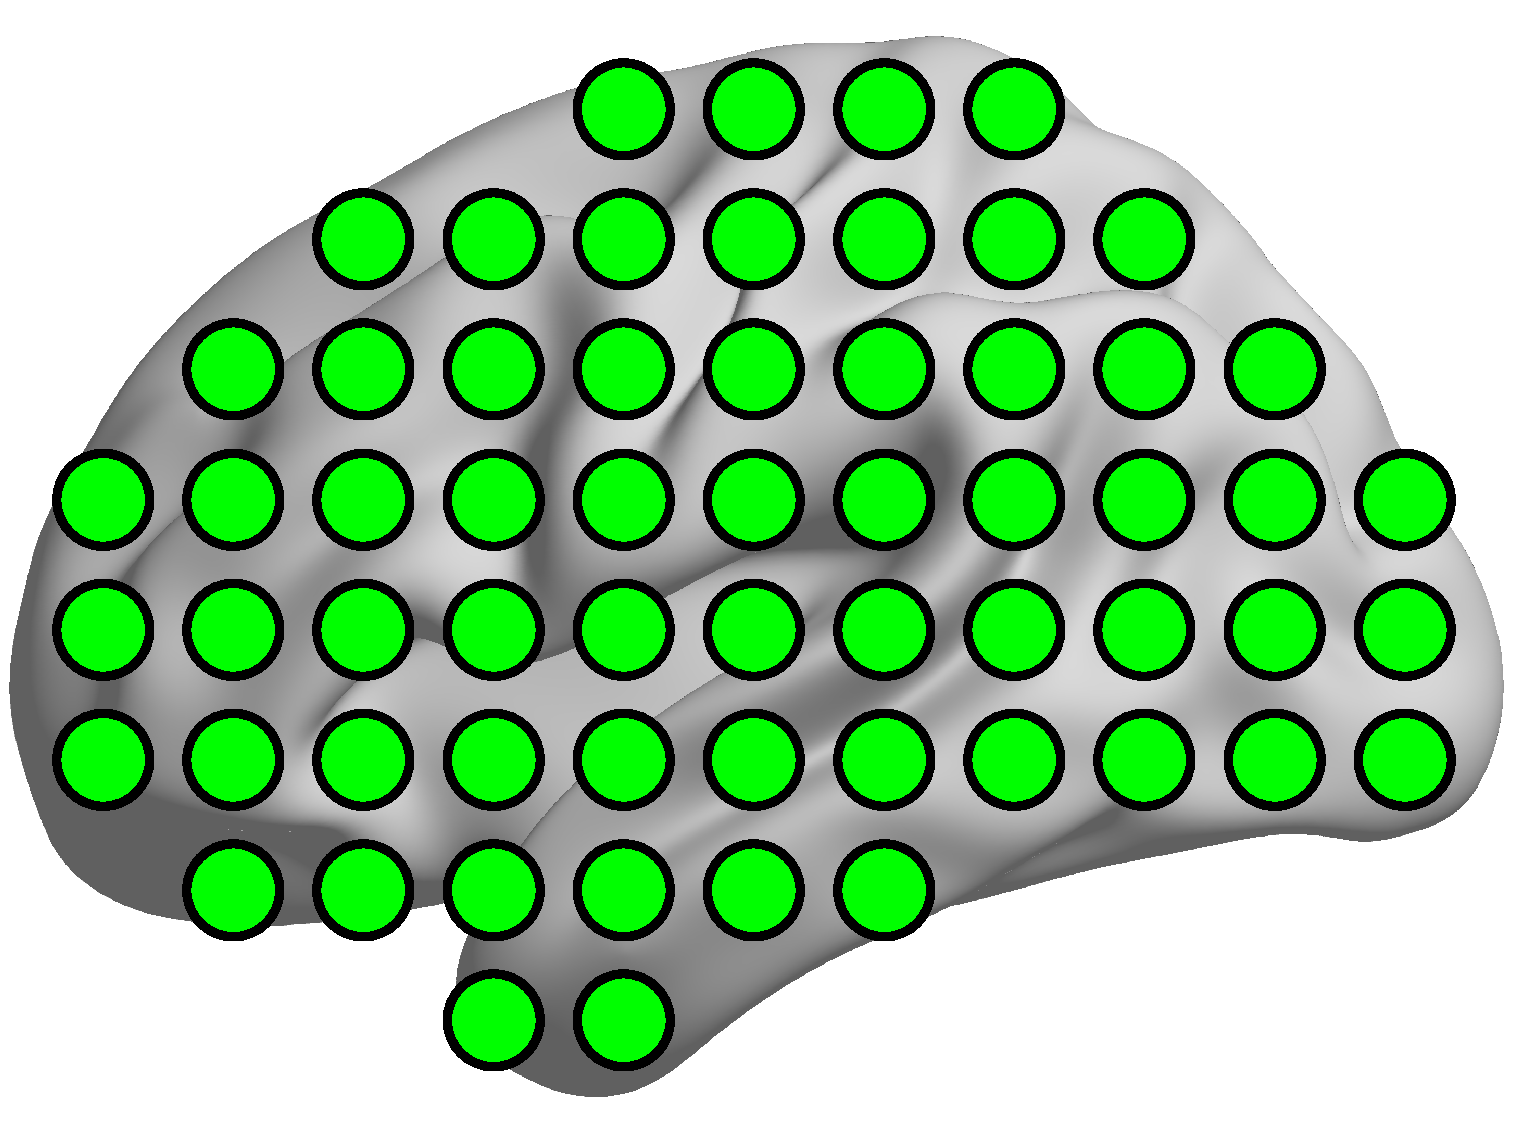
\includegraphics[width=0.85\linewidth]{\fig/brain_seed_placement_FOV.pdf}}
			}_\x
		$
		\caption{Original Functional connectome}
	\end{subfigure}
	\hspace{0.05\linewidth}
	\begin{subfigure}[t]{\imwidth}
		\centering
		{\Large
		$\underbrace{
			\myfbox{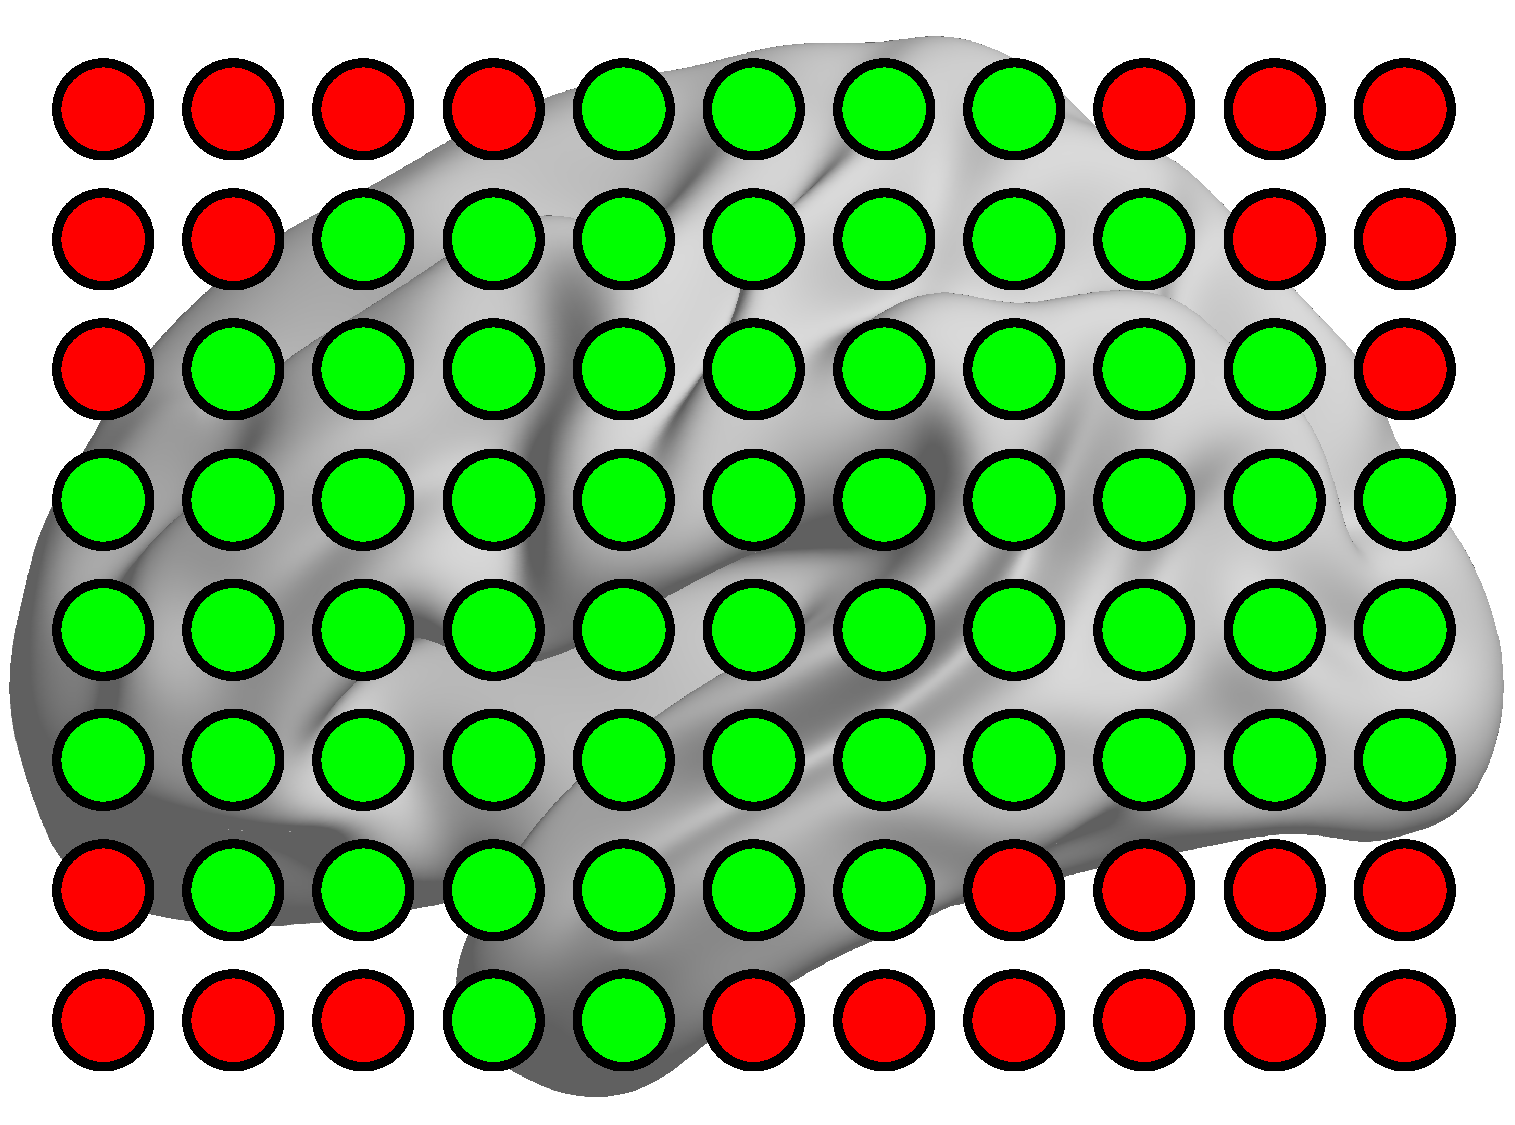
\includegraphics[width=0.85\linewidth]{\fig/brain_seed_placement_all.pdf}}
			}_{\xstar=\A_1\x}
		$}
		\caption{Intermediate augmented connectome}
	\end{subfigure}
	\caption{
		The effect of the first level augmentation matrix $\A_1$.
		\textbf{Left:} the original functional connectome \x only contains edges between the nodes placed on the support of the brain (represented by the green nodes).
		\textbf{Right:}
		$\A_1$ pads extra zero entries on \x to create the intermediate augmented connectome \xstar.
		Here, \xstar can be treated as if the nodes were placed throughout the entire rectangular FOV (the red bubbles represent nodes that are outside the brain support), as its entries contain all possible edges between the green and red nodes; the edges that connect with the red nodes all have zero values. 
	}\label{fig:augmat1}\vspace{0.025\linewidth}
	\renewcommand{\VSPACE}{\vspace{-0.135in}}
	\begin{subfigure}[b]{0.39\linewidth}
		\centering
		\small
		\(
\xstar = \ba{c} \xstar(\r_2,\r_1) \\ \xstar(\r_3,\r_1) \\ \vdots \\ \xstar(\r_d,\r_1) \\ \hline \VSPACE \\
\xstar(\r_3,\r_2) \\ \xstar(\r_4,\r_2) \\ \vdots \\ \xstar(\r_d,\r_2) \\ \hline
\vdots \\ \hline \VSPACE \\  \xstar(\r_d,\r_{d-1})  \ea,
		\)
		\vspace{8pt}
		\caption{Intermediate augmented connectome}
	\end{subfigure}
	\begin{subfigure}[b]{0.6\linewidth}
		\small\centering
		\(
\xtil=\A_2\xstar
=
\ba{c} \dored{\xtil(\r_1,\r_1)} \\ \xtil(\r_2,\r_1) \\ \xtil(\r_3,\r_1) \\ \vdots \\ \xtil(\r_{d},\r_1) \\ \hline \VSPACE \\  
\dored{\xtil(\r_1,\r_2)} \\ \dored{\xtil(\r_2,\r_2)} \\ \xtil(\r_3,\r_2) \\ \vdots \\ \xtil(\r_{d},\r_2) \\ \hline \vdots \\ \dored{\xtil(\r_{d},\r_{{d}})}  \ea
=
\ba{c} \dored{0} \\ \xstar(\r_2,\r_1) \\ \xstar(\r_3,\r_1) \\ \vdots \\ \xstar(\r_{d},\r_1) \\ \hline \VSPACE \\ \dored{0} \\ \dored{0} \\ \xstar(\r_3,\r_2) \\ \vdots \\ \xstar(\r_{d},\r_2) \\ \hline \vdots \\ \dored{0}  \ea
		\)
		\caption{Augmented functional connectome}
	\end{subfigure}
	\caption{
		The effect of the second level augmentation matrix $\A_2$.  
		The entries of \xstar represent edges localized by $6$-D coordinate points $\left\{(\r_j,\r_k) \; |\;  j>k\right\}$, where $\r_j=(x_j,y_j,z_j)$ and $\r_k=(x_k,y_k,z_k)$ are the $3$-D locations of the node pairs defining the edges.
		$\A_2$ fixes the asymmetry in the coordinates of \xstar by padding zero entries to accommodate for the $6$-D coordinate points $\left\{(\r_j,\r_k) \; |\;  j\leq k\right\}$; these are the diagonal and the upper-triangular entries in the cross-correlation matrix that were disposed for redundancy.
	}
	\label{fig:augmat2}
\end{figure}
%*************************************************************************%

%===================================================================%
% ADMM algorithm for elastic net
%===================================================================%
\section{ADMM updates for Elastic-net}
\label{appendix,admm,enet}
The unconstrained formulation of the Elastic-net regularized ERM problem reads
\begin{equation}
	\argmin{\w\in\reals^p} \frac{1}{n}\Loss(\YXw) + \lambda\norm{\w}_1 + \frac{\gamma}{2}\norm{\w}^2_2 \;,
	\nonumber
\end{equation}
which can be converted into the following equivalent constrained formulation:
\begin{equation}
	\begin{array}{c}
		\dstyle\minimize{\w,\va \vb}
			\frac{1}{n}\Loss(\va)+\lambda\norm{\vb}_1+ \frac{\gamma}{2}\norm{\w}^2_2 \;
			\vspace{0.01\linewidth}
		\text{ subject to }  \YXw =\va, \; \w=\vb \;.
	\end{array}
	\label{eqn:splitting,enet}
\end{equation}
With this variable splitting scheme, the correspondence with the ADMM formulation~\eqref{eqn:canonical,admm} is
\begin{equation}
	\begin{array}{c}
		\fbar(\xbar)=\frac{\gamma}{2}\norm{\w}^2_2 , \;\;\;
		\gbar(\ybar)=\dstyle\frac{1}{n}\Loss(\va) + \lambda\norm{\vb}_1  
		\vspace{0.02\linewidth} \\
		\Abar = 	\ba{cc} 	\Y\X	 \\ \I \ea 	, \quad
		\xbar = \w, \quad
		\Bbar = 	-\I		, \quad
		\ybar = \bmat \va \\ \vb \emat \;.
		\end{array}
	\nonumber
\end{equation}
and the ADMM updates for \xbar~\eqref{eqn:admm,xbar,update} and \ybar~\eqref{eqn:admm,ybar,update} decomposes into subproblems
\begin{alignat}{1} 
	\w\iterp 	\leftarrow \argmin{\w}&
		 \Bigg\{ \frac{\gamma}{2}\norm{\w}^2
		+ \normsq{\Y\X\w-\left(\va\iter-\ua\iter\right)} 
		+ \normsq{\w-\left(\vb\iter-\ub\iter\right)} \Bigg\} \nonumber \\
	\va\iterp \leftarrow \argmin{\va}
		& \left\{ \frac{1}{n}\Loss(\va) + \frac{\rho}{2}\normsq{\va-\left(\Y\X\w\iterp+\ua\iter\right)} \right\}
			\nonumber \\
	\vb\iterp \leftarrow \argmin{\vb} 
		& \left\{\lambda\norm{\vb}_1 + \frac{\rho}{2}\normsq{\vb-\left(\w\iterp+\ub\iter\right)} 
			\nonumber\right\} \;.
\end{alignat}
The update for \w is
\begin{align}
	\w\iterp \leftarrow \left(\rho\X^T\X + [\gamma+\rho]\BI_p\right)\inv  
		\Big(&\rho\X^T\Y^T [\va\iter-\ua\iter] 
		+\rho[\vb\iter-\ub\iter] \Big) \, \nonumber
\end{align} which can be solved efficiently via inversion Lemma \eqref{eqn:inv,lemma}.
The update for \va and \vb is identical to \eqref{eqn:v1,update1} and \eqref{eqn:v2,update1} described in Sec.~\ref{subsec:admm,steps}, which can be solved via coordinate-wise proximal operators \eqref{eqn:v1,update2} and \eqref{eqn:v2,update2}.
The dual variable update \eqref{eqn:admm,dual,update} is a trivial matrix-vector multiplication.
